\documentclass[a4paper,14pt]{extarticle}

% Путь до папки с общими шаблонами
\newcommand{\pathToCommonFolder}{/home/denilai/Documents/repos/latex/Common}
% Название работы в титуле
\newcommand{\workname}{Практическая работа №1}
% Название дисциплины в титуле
\newcommand{\discipline}{Техническое обслуживание\\программно--аппаратных комплексов}
% Название кафедры в титуле
\newcommand{\kafedra}{Кафедры Вычислительной техники}
% Тема работы в титуле
\newcommand{\theme}{}
\newcommand{\dontneedtheme}{1}
% Должность преподавателя в титуле
\newcommand{\rang}{ассистент, }
% ФИО студента в титуле
\newcommand{\studentfio}{К.~Ю.~Денисов}
% ФИО преподавателя в титуле
\newcommand{\teacherfio}{Л.~В.~Скоропупов}
\newcommand{\signature}{\pathToCommonFolder/empty}

\usepackage{tabularx}


\usepackage{booktabs}
%\newcolumntype{b}{X}
%\newcolumntype{s}{>{\hsize=.5\hsize}X}
\newcommand{\heading}[1]{\multicolumn{1}{c}{#1}}

% установка размера шрифта для всего документа
%\fontsize{20pt}{18pt}\selectfont
\usepackage{extsizes} % Возможность сделать 14-й шрифт

% Вставка заготовки преамбулы
% Этот шаблон документа разработан в 2014 году
% Данилом Фёдоровых (danil@fedorovykh.ru) 
% для использования в курсе 
% <<Документы и презентации в \LaTeX>>, записанном НИУ ВШЭ
% для Coursera.org: http://coursera.org/course/latex .
% Исходная версия шаблона --- 
% https://www.writelatex.com/coursera/latex/5.3

% В этом документе преамбула

% Для корректного использования русских символов в формулах
% пакеты hyperref и настройки, связанные с ним, стоит загуржать
% перед загрузкой пакета mathtext



% поддержка русских букв
% кодировка шрифта
%\usepackage[T2A]{fontenc} 
\usepackage{pscyr}

% использование ненумеровонного абзаца с добавлением его в содержаниеl

\newcommand{\anonsection}[1]{\section*{#1}\addcontentsline{toc}{section}{#1}}
\newcommand{\sectionunderl}[1]{\section*{\underline{#1}}}


% настройка окружения enumerate
\usepackage{enumitem}
\setlist{noitemsep}
\setlist[enumerate]{labelsep=*, leftmargin=1.5pc}

\usepackage{hyperref}

% сначала ставить \usepackage{extsizes} % Возможность сделать 14-й шрифт
% для корректной установки полей вставлять преамбулу следует в последнюю очередь (но перед дерективой замены \rmdefault)
\usepackage[top=20mm,bottom=25mm,left=35mm,right=20mm]{geometry} % Простой способ задавать поля

\hypersetup{				% Гиперссылки
	unicode=true,           % русские буквы в раздела PDF
	pdftitle={Заголовок},   % Заголовок
	pdfauthor={Автор},      % Автор
	pdfsubject={Тема},      % Тема
	pdfcreator={Создатель}, % Создатель
	pdfproducer={Производитель}, % Производитель
	pdfkeywords={keyword1} {key2} {key3}, % Ключевые слова
	colorlinks=true,       	% false: ссылки в рамках; true: цветные ссылки
	linkcolor=red,          % внутренние ссылки
	citecolor=black,        % на библиографию
	filecolor=magenta,      % на файлы
	urlcolor=blue           % на URL
}

%%% Работа с русским языком
\usepackage{cmap}					% поиск в PDF
\usepackage{mathtext} 				% русские буквы в формулах
\usepackage[T2A]{fontenc}			% кодировка
\usepackage[utf8]{inputenc}			% кодировка исходного текста
\usepackage[english,russian]{babel}	% локализация и переносы
\usepackage{indentfirst}
\frenchspacing

%для изменения названия списка иллюстраций
\usepackage{tocloft}


\renewcommand{\epsilon}{\ensuremath{\varepsilon}}
\renewcommand{\phi}{\ensuremath{\varphi}}
\renewcommand{\kappa}{\ensuremath{\varkappa}}
\renewcommand{\le}{\ensuremath{\leqslant}}
\renewcommand{\leq}{\ensuremath{\leqslant}}
\renewcommand{\ge}{\ensuremath{\geqslant}}
\renewcommand{\geq}{\ensuremath{\geqslant}}
\renewcommand{\emptyset}{\varnothing}

% Изменения параметров списка иллюстраций
\renewcommand{\cftfigfont}{Рисунок } % добавляем везде "Рисунок" перед номером
\addto\captionsrussian{\renewcommand\listfigurename{Список иллюстративного материала}}

\newcommand{\tm}{\texttrademark\ }
\newcommand{\reg}{\textregistered\ }


%%% Дополнительная работа с математикой
\usepackage{amsmath,amsfonts,amssymb,amsthm,mathtools} % AMS
\usepackage{icomma} % "Умная" запятая: $0,2$ --- число, $0, 2$ --- перечисление

%% Номера формул
%\mathtoolsset{showonlyrefs=true} % Показывать номера только у тех формул, на которые есть \eqref{} в тексте.
%\usepackage{leqno} % Нумереация формул слева

%% Свои команды
\DeclareMathOperator{\sgn}{\mathop{sgn}}

%% Перенос знаков в формулах (по Львовскому)
\newcommand*{\hm}[1]{#1\nobreak\discretionary{}
{\hbox{$\mathsurround=0pt #1$}}{}}


% отступ для первого абзаца главы или параграфа
%\usepackage{indentfirst}

%%% Работа с картинками
\usepackage{graphicx}  % Для вставки рисунков
\graphicspath{{images/}{screnshots/}}  % папки с картинками
\DeclareGraphicsExtensions{.pdf,.png,.jpg}
\setlength\fboxsep{3pt} % Отступ рамки \fbox{} от рисунка
\setlength\fboxrule{1pt} % Толщина линий рамки \fbox{}
\usepackage{wrapfig} % Обтекание рисунков текстом

%%% Работа с таблицами
\usepackage{array,tabularx,tabulary,booktabs} % Дополнительная работа с таблицами
\usepackage{longtable}  % Длинные таблицы
\usepackage{multirow} % Слияние строк в таблице

%%% Теоремы
\theoremstyle{plain} % Это стиль по умолчанию, его можно не переопределять.
\newtheorem{theorem}{Теорема}[section]
\newtheorem{proposition}[theorem]{Утверждение}

\theoremstyle{plain} % Это стиль по умолчанию, его можно не переопределять.
\newtheorem{work}{Практическая работа}[part]


 
 
\theoremstyle{definition} % "Определение"
\newtheorem{corollary}{Следствие}[theorem]
\newtheorem{problem}{Задача}[section]
 
\theoremstyle{remark} % "Примечание"
\newtheorem*{nonum}{Решение}



%%% Программирование
\usepackage{etoolbox} % логические операторы

%%% Страница

%	\usepackage{fancyhdr} % Колонтитулы
% 	\pagestyle{fancy}
%   \renewcommand{\headrulewidth}{0pt}  % Толщина линейки, отчеркивающей верхний колонтитул
% 	\lfoot{Нижний левый}
% 	\rfoot{Нижний правый}
% 	\rhead{Верхний правый}
% 	\chead{Верхний в центре}
% 	\lhead{Верхний левый}
%	\cfoot{Нижний в центре} % По умолчанию здесь номер страницы

\usepackage{setspace} % Интерлиньяж
\onehalfspacing % Интерлиньяж 1.5
%\doublespacing % Интерлиньяж 2
%\singlespacing % Интерлиньяж 1

\usepackage{lastpage} % Узнать, сколько всего страниц в документе.

\usepackage{soul} % Модификаторы начертания


\usepackage[usenames,dvipsnames,svgnames,table,rgb]{xcolor}


\usepackage{csquotes} % Еще инструменты для ссылок

%\usepackage[style=authoryear,maxcitenames=2,backend=biber,sorting=nty]{biblatex}

\usepackage{multicol} % Несколько колонок

\usepackage{tikz} % Работа с графикой
\usepackage{pgfplots}
\usepackage{pgfplotstable}

% модуль для вставки рыбы
\usepackage{blindtext}

\usepackage{listings}
\usepackage{color}


% для поворота отдельной страницы. Использовать окружение \landscape
\usepackage{pdflscape} 
\usepackage{rotating} 


\definecolor{mygreen}{rgb}{0,0.6,0}
\definecolor{mygray}{rgb}{0.5,0.5,0.5}
\definecolor{mymauve}{rgb}{0.58,0,0.82}


% пример импорта файла
%\lstinputlisting{/home/denilai/repomy/conf/distributions}

\lstset{
	language=Python,
	basicstyle=\footnotesize,        % the size of the fonts that are used for the code
	numbers=left,                    % where to put the line-numbers; possible values are (none, left, right)
	numbersep=5pt,                   % how far the line-numbers are from the code
	numberstyle=\tiny\color{mygray}, % the style that is used for the line-numbers
	stepnumber=2,                    % the step between two line-numbers. If it's 1, each line will be numbered
	% Tab - 2 пробела
	tabsize=2,    
	% Автоматический перенос строк
	breaklines=true,
	frame=single,
	breakatwhitespace=true,
	title=\lstname 
}


%\usepackage[top=20mm,bottom=20mm,left=20mm,right=15mm]{geometry} % Простой способ задавать поля

\author{Кирилл Денисов}
\title{Практическая работа №4}
\date{\today}

\renewcommand{\withouttheme}{1}

% установка полуторного интервала
% \usepackage{setspace}  
% \onehalfspacing

% использовать Times New Roman
\renewcommand{\rmdefault}{ftm}


\begin{document}
	\thispagestyle{empty}
	% Вставка первого титульного листа
	%\newcommand{\withouttheme}{} добавить эту переменную для определения, нужна ли тема
%     {} - нужна
%    {1} - не нужна

%\newcommand{\withoutsubmissiondate}{} добавить эту переменную для определения, нужен ли срок предоставления отчета
%     {} - нужен
%    {1} - не нужен
\begin{center}
	\begin{figure}[h!]
		\begin{center}
		
\includegraphics[width=0.17\linewidth]{\pathToCommonFolder/gerb}
		%\caption{}\label{pic:first}
		%	\vspace{5ex}
		\end{center}	
	\end{figure}
 	\small	МИНОБРНАУКИ РОССИИ \\
	Федеральное государственное бюджетное образовательное учреждение\\
						высшего профессионального образования\\
\normalsize					
\textbf{«МИРЭА – Российский технологический университет»\\
						РТУ МИРЭА}\\
						\noindent\rule{1\linewidth}{1pt}\\
       Институт информационных технологий\\ %\vspace{2ex}
					\kafedra\\
		\vspace{3ex}
			\large \textbf{\workname}  \\
		%\vspace{1ex}
						по дисциплине\\ «\discipline» \\
		\vspace{3ex}
		\if \withouttheme
			\textbf{Тема работы:}\\ <<\theme>>
		\fi
\vspace{3ex}
\small
\begin{table}[h!]
\begin{tabular}{p{0.14\linewidth}p{0.38\linewidth}p{0.25\linewidth}p{0.2\linewidth}}
	\textbf{Выполнил:} & студент группы ИВБО-02-19 & \studentfio &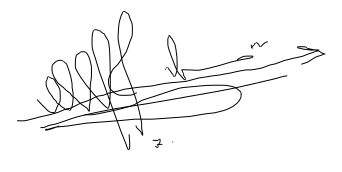
\includegraphics[width=0.8\linewidth]{\signature}\\ \\
	\textbf{Принял:} & \rang & \teacherfio 
\end{tabular}
\end{table}
\end{center}

\begin{flushleft}
	\begin{tabular}{p{0.25\linewidth}l}

		Работа выполена & <<\noindent\rule{2em}{1pt}>>
		                    \noindent\rule{5em}{1pt} 202\noindent\rule{1em}{1pt} \\

		<<Зачтено>> & <<\noindent\rule{2em}{1pt}>>
		\noindent\rule{5em}{1pt} 202\noindent\rule{1em}{1pt} \\

	\end{tabular}
\end{flushleft}

\normalsize
\begin{center}	
\vfill 
Москва 2021
\end{center}

	\newpage
%	\tableofcontents
	\newpage
%	\listoftables
	
	
	
	
\section*{Постановка задачи}

Составить календарный график работ еженедельного, ежемесячного, полугодового профилактического обслуживания, согласно варианту.

\section*{Теоретические сведения} 

Эксплуатация средств ВТ заключается в использовании их для выполнения всего комплекса возложенных на него задач. Для эффективного использования и поддержания ЭВМ и других средств ВТ в работоспособном состоянии в процессе эксплуатации должно проводиться техническое обслуживание.

\textbf{Техническое обслуживание} --- это комплекс организационных мероприятий в том числе обеспечение средств ВТ необходимой аппаратурой и оборудованием предназначенной для эффективной эксплуатации.

Что включает в себя профилактика
\begin{enumerate}
\item Чистка от загрязнений --- внутри и снаружи. Пыль забивается в вентиляционные отверстия системного блока, попадает на материнскую плату и комплектующие. Если долго не чистить ПК изнутри --- он начнёт перегреваться, и однажды что-нибудь «полетит». И да, клавиатуру и монитор тоже надо чистить.

\item  Проверка работоспособности компонентов. Нужно оценить, как работают процессор и видеокарта, нет ли проблем с блоком питания, звуковой и сетевой картами и т.д. Лучше найти и устранить неполадки, когда они только начинают проявляться.

\item  Проверка производительности системы. ОС тоже регулярно надо чистить от мусора: «остатков» удалённых программ, ненужных файлов, вирусов (которые часто просачиваются, даже если работает хороший корпоративный антивирус). Всё это улучшает быстродействие --- компьютер меньше тормозит и не виснет при большой загруженности.

\item  Апгрейд программного обеспечения. Разработчики не зря выпускают обновленные версии программ --- там исправлены баги и недоработки предыдущих версий.

\item  Проверка работы антивирусной системы. Антивирус должен работать беспрерывно, а базы --- регулярно обновляться.

\item  Резервное копирование. Обычно копии важных данных создаются автоматически, но иногда необходимо ручное копирование.
\end{enumerate}

\subsubsection*{Основные эксплуатационные характеристики}

Степень пригодности ВС к использованию по назначению определяется эксплуатационными характеристиками.

Под \textit{работоспособностью} средств ВТ понимается способность ВТ функционировать, обеспечивая выполнение заданных функций с параметрами, установленными требованиям их документации. Эта характеристика позволяет судить о состоянии ВТ в определенный момент времени, однако, при эксплуатации важно знать её состояние не только в данный момент времени, но и способность выполнять возложенные задачи в течение заданного промежутка времени. Для этих целей вводится понятие безотказность.

Под \textit{безотказностью} средств ВТ понимают её способность сохранять работоспособность в течение заданного интервала времени при определенных условиях эксплуатации.

На этапе хранения средств ВТ пользуются такой характеристикой как \textit{сохранность}, под которой понимают способность ВТ сохранять исправное состояние при заданных условиях хранения.

Для характеристики ВТ с точки зрения ее приспособленности к ремонту вводится понятие \textit{ремонтопригодности}.

Под \textit{долговечностью} понимают свойства средств ВТ сохранять работоспособность для определенного состояния с необходимыми перерывами для технического обслуживания и ремонтов.

Важной характеристикой является \textit{надежность}.

\subsubsection*{Принципы организации эксплуатации}

Эффективность использования средств ВТ во многом зависит от того насколько рационально организована эксплуатация данных средств. В целом организация эксплуатации включает в себя:
\begin{itemize}[label=--]
\item Выбор системы обслуживания;

\item Материальное обеспечение обслуживания средств ВТ;

\item Определение необходимого количества обслуживающего персонала и его квалификации;

\item Планово-профилактические работы;

\item Эксплуатационная документация;

\item Планирование эксплуатации средств ВТ;

\item Анализ и учет результатов эксплуатации;

\item Организация и систематическое обучение обслуживающего персонала.
\end{itemize}

\paragraph{Материальное обеспечение обслуживания.} Качество эксплуатации средств ВТ зависит от обеспечения ее запасными элементами, различными приспособлениями и расходными материалами. Обеспечение контрольно-измерительными приборами и инструментами.

\paragraph{Эксплуатационная документация.} Её состав зависит от класса вычислительных машин, состава оборудования и т. д. В состав могут быть включены: формуляры, техническое описание, инструкция по эксплуатации и т.~д.

\paragraph{Планирование эксплуатации.} Планирование является основой рациональной организации эксплуатации средств ВТ. Оно служит для определения конкретной программы действий на какой-либо календарный срок. Различают следующие виды планирования:

\begin{itemize}
\item Оперативно-календарное. Заключается в составлении планов загрузки машины и работы обслуживающего персонала исходя из объемов запросов машинного времени. Планирование машинного времени возможно только на 7-10 дней вперед.

\item Планирование организационно-технических мероприятий заключается в составлении программы работы обслуживающего персонала.

\end{itemize}

\paragraph{Анализ и учет результатов эксплуатации.} В процессе эксплуатации ВТ необходимо вести учет - журналы эксплуатации средств ВТ и журнал учета машинного времени

\paragraph{Техническое обслуживание компьютеров.} Для того, чтобы Ваш компьютер работал без сбоев необходимо периодически проводить техническое обслуживание. К техническому обслуживанию можно отнести:

\begin{itemize}
\item Механические операции очистки компонентов компьютера от грязи и пыли;

\item Операции, связанные с защитой операционной системы;

\item Операции периодической очистки от неиспользуемых программ.
\end{itemize}


\section*{Ход работы}

\textbf{Индивидуальный вариант №6}
\begin{table}[htbp]
	    \caption{Индивидуальный вариант №6}
	\small
	\begin{tabular}{|p{0.1\linewidth}|p{0.12\linewidth}|p{0.12\linewidth}|p{0.12\linewidth}|p{0.12\linewidth}|p{0.12\linewidth}|p{0.12\linewidth}|}
		\hline
		№
		Варианта & Кол-во
		ПК & Кол-во
		лазерных
		принтеров & Кол-во
		струйных
		принтеров & Текущий ремонт & Научно-технические услуги & Заказ и получение оборудования \\ \hline
		\multicolumn{1}{|r|}{6} & \multicolumn{1}{r|}{4} & \multicolumn{1}{r|}{1} & \multicolumn{1}{r|}{1} & \multicolumn{1}{r|}{0} & \multicolumn{1}{r|}{2} & \multicolumn{1}{r|}{1} \\ \hline
	\end{tabular}

	\label{}
\end{table}
\newpage
\section*{График технического обслуживания}

\subsection*{График еженедельного технического обслуживания}
	\begin{table}[htbp]
			\caption{График еженедельного технического обслуживания}
	\centering
	\small
	\begin{tabular}{|p{0.75\linewidth}|m{0.23\linewidth}|}
		\hline
		\multicolumn{1}{|c|}{Наименование работы} & Длительность (ч) \\ \hline
		\multicolumn{ 2}{|l|}{Еженедельное} \\ \hline
		\multicolumn{ 2}{|c|}{ПК-1, ПК-2, ПК-3, ПК-4} \\ \hline
		Проверка работоспособности устройств на тестах в ускоренном режиме  & 0.52 \\ \hline
		Очистка магнитных головок устройств внешней памяти (накопители на гибких магнитных дисках (НГМД))  & 0.36 \\ \hline
		Проверка и удаление компьютерных вирусов на устройствах внешней памяти ПЭВМ  & 0.8 \\ \hline
		Проведение дефрагментации накопителей на жестких магнитных дисках  & 1.08 \\ \hline
		Проверка линий и устройств локальной вычислительной сети с помощью автономных тестов  & 0.76 \\ \hline
		\multicolumn{ 2}{|c|}{НТУ-1, НТУ-2} \\ \hline
		Генерация конкретных вариантов ПС ПЭВМ из дистрибутивной МЛ, поставленной пользователю под параметры ПЭВМ & 15 \\ \hline
		\multicolumn{ 2}{|c|}{ЗПО-1} \\ \hline
		Получение еженедельных заказов на оборудование  & 0.15 \\ \hline
		Составление списка заказов на оборудование  & 0.1 \\ \hline
		Получение разрешения уполномоченного лица на получение оборудования  & 0.15 \\ \hline
		Проверка оплаты заказа  & 0.1 \\ \hline
		Передача списка заказов на оборудование на склад  & 0.15 \\ \hline
		Получение оборудования со склада  & 0.8 \\ \hline
		Получение счета - фактуры на заказанное оборудование  & 0.18 \\ \hline
		Подготовка отчетных данных по заказам  & 0.7 \\ \hline
		\multicolumn{ 2}{|c|}{ПС-1} \\ \hline
		Проверка работоспособности устройств на тестах в ускоренном режиме & 0.13 \\ \hline
	\end{tabular}

	\label{tab:week}
\end{table}
\newpage
\subsection*{График ежемесячного технического обслуживания}
	\small
	\begin{longtable}{|p{0.75\linewidth}|m{0.23\linewidth}|}
	
			\caption{График ежемесячного технического обслуживания}
		\endfirsthead
		
		%\hline
		\multicolumn{2}{c}{\textit{Продолжение таблицы \ref{tab:month}}}
		%\hline
		\endhead
		
		\hline
		\endfoot
		
		
		%\multicolumn{2}{c}{\textit{Конец таблицы \ref{tab:month}}}\\
		\endlastfoot
		
		
		\hline
		\multicolumn{1}{|c|}{Наименование работы} & Длительность работы (час) \\ \hline
		\multicolumn{ 2}{|c|}{Ежемесячное} \\ \hline
		\multicolumn{ 2}{|c|}{ПК-1, ПК-2, ПК-3, ПК-4} \\ \hline
		\multicolumn{1}{|l|}{Еженедельное ТО ПК-1, ПК-2, ПК-3, ПК-4} & 14.08 \\ \hline
		Полное тестирование всех устройств ПЭВМ с выдачей протокола, в том числе и ЛВС, выявление и исправление ошибок в распределении дискового пространства  & 4.7 \\ \hline
		Поставка обновленных антивирусных программ и полная проверка дисковой памяти на наличие вирусов  & 1.7 \\ \hline
		Смазка механических устройств НГМД, стримеры, принтеры  & 1.36 \\ \hline
		Очистка от пыли внутренних объемов ПЭВМ с разборкой  & 1 \\ \hline
		Очистка от пыли и грязи видеомониторов, регулировка и настройка  & 1.4 \\ \hline
		\multicolumn{ 2}{|c|}{ПЛ-1} \\ \hline
		Смазка механических устройств НГМД, стримеры, принтеры  & 0.34 \\ \hline
		Очистка от использованного тонера элементов печати лазерных принтеров, очистка и промывка оптики и заправка тонера  & 0.37 \\ \hline
		\multicolumn{ 2}{|c|}{ПС-1} \\ \hline
		Смазка механических устройств НГМД, стримеры, принтеры  & 0.35 \\ \hline
		Очистка и промывка печатающих головок матричных и струйных принтеров  & 0.17 \\ \hline
		Ремонт струйных принтеров  & 1.8 \\ \hline
		\multicolumn{ 2}{|c|}{НТУ-1, НТУ-2} \\ \hline
		Проверка установленных лент временной корректировки программ  & 4.7 \\ \hline
		\multicolumn{ 2}{|c|}{ЗПО-1} \\ \hline
		Получение еженедельных заказов на оборудование  & 0.15 \\ \hline
		Составление списка заказов на оборудование  & 0.1 \\ \hline
		Получение разрешения уполномоченного лица на получение оборудования  & 0.15 \\ \hline
		Проверка оплаты заказа  & 0.1 \\ \hline
		Передача списка заказов на оборудование на склад  & 0.15 \\ \hline
		Получение оборудования со склада  & 0.8 \\ \hline
		Получение счета - фактуры на заказанное оборудование  & 0.18 \\ \hline
		Подготовка отчетных данных по заказам  & 0.7 \\ \hline

		\label{tab:month}
	\end{longtable}

\normalsize
\subsection*{График полугодового (включая еженедельное и ежемесячное) технического обслуживания}
\small
\begin{longtable}{|p{0.75\linewidth}|m{0.23\linewidth}|}

		\caption{График полугодового технического обслуживания}
\endfirsthead

%\hline
\multicolumn{2}{c}{\textit{Продолжение таблицы \ref{tab:year}}}\\
%\hline
\endhead

\hline
\endfoot


%\multicolumn{2}{c}{\textit{Конец таблицы \ref{tab:month}}}\\
\endlastfoot
		\hline
		\multicolumn{1}{|c|}{Наименование работы} & Длительность работы (час) \\ \hline
		\multicolumn{ 2}{|c|}{Полугодовое} \\ \hline
		\multicolumn{ 2}{|c|}{ПК-1, ПК-2, ПК-3, ПК-4} \\ \hline
		\multicolumn{1}{|c|}{Ежемесячное ТО ПК-1, ПК-2, ПК-3, ПК-4} & 339.36 \\ \hline
		Очистка от пыли внутренних объемов 
		блоков питания ПЭВМ, очистка и 
		смазка вентиляторов  & 3.2 \\ \hline
		Очистка экранов видеомониторов и LCD 
		панели от пыли и грязи, регулировка 
		и настройка  & 0.88 \\ \hline
		Очистка от пыли внутренних объемов 
		внешних модемов, устройств 
		независимого питания (UPS) с 
		последующим их тестированием  & 1.88 \\ \hline
		\multicolumn{ 2}{|c|}{ЛП-1} \\ \hline
		Ежемесячное ТО ЛП-1 & 8.76 \\ \hline
		Очистка от пыли внутренних объемов внешних модемов, устройств независимого питания (UPS) с последующим их тестированием & 0.47 \\ \hline
		\multicolumn{ 2}{|c|}{ПС-1} \\ \hline
		Ежемесячное ТО ЛП-1 & 2.32 \\ \hline
		Замена печатающих головок матричных и струйных принтеров теров  & 1.8 \\ \hline
		\multicolumn{ 2}{|c|}{НТУ-1, НТУ-2} \\ \hline
		Занесение в форму запроса деталей об 
		ошибке или изменении   & 1.6 \\ \hline
		\multicolumn{ 2}{|c|}{ЗПО-1} \\ \hline
		Получение еженедельных заказов на 
		оборудование  & 0.15 \\ \hline
		Составление списка заказов на 
		оборудование  & 0.1 \\ \hline
		Получение разрешения уполномоченного 
		лица на получение оборудования  & 0.15 \\ \hline
		Проверка оплаты заказа  & 0.1 \\ \hline
		Передача списка заказов на 
		оборудование на склад  & 0.15 \\ \hline
		Получение оборудования со склада  & 0.8 \\ \hline
		Получение счета - фактуры на 
		заказанное оборудование  & 0.18 \\ \hline
		Подготовка отчетных данных по 
		заказам  & 0.7 \\ \hline

		\label{tab:year}
	\end{longtable}



\newpage
\section*{Календарный план проведения технического обслуживания}
\subsection*{Календарный план проведения еженедельного технического обслуживания}


	\begin{longtable}{|p{0.35\linewidth}|p{0.1\linewidth}|p{0.1\linewidth}|p{0.13\linewidth}|p{0.17\linewidth}|}
	
			\caption{Календарный план проведения еженедельного технического обслуживания}
	\endfirsthead
	
	%\hline
	\multicolumn{5}{c}{\textit{Продолжение таблицы \ref{tab:calendar-week}}}\\
	%\hline
	\endhead
	
	\endfoot
	
	
	%\multicolumn{2}{c}{\textit{Конец таблицы \ref{tab:month}}}\\
	\endlastfoot
		\hline
		\multicolumn{1}{|c|}{Наименование работы} & Дата & Начало & Окончаниe & Исполнитель \\ \hline
		\multicolumn{ 5}{|c|}{Еженедельное} \\ \hline
		\multicolumn{ 5}{|c|}{ПК-1, ПК-2, ПК-3, ПК-4} \\ \hline
		Проверка работоспособности устройств на тестах в ускоренном режиме  & 10.01.21 & 09:00 & 09:31 & Денисов К.Ю. \\ \hline
		Очистка магнитных головок устройств внешней памяти (накопители на гибких магнитных дисках (НГМД))  & 10.01.21 & 09:31 & 09:52 & Денисов К.Ю. \\ \hline
		Проверка и удаление компьютерных вирусов на устройствах внешней памяти ПЭВМ  & 10.01.21 & 09:52 & 10:40 & Денисов К.Ю. \\ \hline
		Проведение дефрагментации накопителей на жестких магнитных дисках  & 10.01.21 & 10:40 & 11:45 & Денисов К.Ю. \\ \hline
		Проверка линий и устройств локальной вычислительной сети с помощью автономных тестов  & 10.01.21 & 11:45 & 12:31 & Денисов К.Ю. \\ \hline
		\multicolumn{1}{|c|}{НТУ-1, НТУ-2} & \multicolumn{ 4}{c|}{} \\ \hline
		Ознакомление с объектом внедрения & 10.01.21 & 15:00 & 16:52 & Денисов К.Ю. \\ \hline
		Разработка рекомендаций по генерации 
		конкретного варианта ОС ПЭВМ из 
		дистрибутивной МЛ поставки и ввод в 
		эксплуатацию сгенерированного ПС  & 11.01.21 & 09:00 & 10:12 & Денисов К.Ю. \\ \hline
		Разработка рекомендаций по 
		составлению технологических 
		инструкций обработки информации, 
		проведение консультаций пользователя 
		в период опытной эксплуатации ПЭВМ  & 11.01.21 & 09:00 & 13:48:00 & Денисов К.Ю. \\ \hline
		Консультации по подготовке 
		пользователями исходных данных в 
		соответствии с требованиями и 
		ограничениями ОС ПЭВМ  & 11.01.21 & 15:00 & 17:00:00 & Денисов К.Ю. \\ \hline
		Разработка рекомендаций по 
		реализации алгоритмов и требований 
		пользователя к обработке данных с 
		использованием ППП ПЭВМ по 
		подготовке задач к опытной 
		эксплуатации  & 12.01.21 & 09:00 & 13:24:00 & Денисов К.Ю. \\ \hline
		Проведение консультаций в процессе 
		опытной эксплуатации задач 
		пользователя  & 12.01.21 & 13:24 & 14:36:00 & Денисов К.Ю. \\ \hline
		\multicolumn{ 5}{|c|}{ЗПО-1} \\ \hline
		Получение еженедельных заказов на оборудование  & 12.01.21 & 15:00 & 15:09 & Денисов К.Ю. \\ \hline
		Составление списка заказов на оборудование  & 12.01.21 & 15:09 & 15:15 & Денисов К.Ю. \\ \hline
		Получение разрешения уполномоченного лица на получение оборудования  & 12.01.21 & 15:15 & 15:24 & Денисов К.Ю. \\ \hline
		Проверка оплаты заказа  & 12.01.21 & 15:24 & 15:30 & Денисов К.Ю. \\ \hline
		Передача списка заказов на оборудование на склад  & 12.01.21 & 15:30 & 15:39 & Денисов К.Ю. \\ \hline
		Получение оборудования со склада  & 12.01.21 & 15:39 & 16:27 & Денисов К.Ю. \\ \hline
		Получение счета - фактуры на заказанное оборудование  & 12.01.21 & 16:27 & 16:37 & Денисов К.Ю. \\ \hline
		Подготовка отчетных данных по заказам  & 12.01.21 & 16:37 & 17:19 & Денисов К.Ю. \\ \hline
		\multicolumn{ 5}{|c|}{ПС-1} \\ \hline
		Проверка работоспособности устройств на тестах в ускоренном режиме & 12.01.21 & 17:19 & 17:27 & Денисов К.Ю. \\ \hline
		\label{tab:calendar-week}
	\end{longtable}

\subsection*{Календарный план проведения ежемесячного технического обслуживания}


	\begin{longtable}{|p{0.35\linewidth}|p{0.1\linewidth}|p{0.1\linewidth}|p{0.13\linewidth}|p{0.17\linewidth}|}
	
			\caption{Календарный план проведения ежемесячного технического обслуживания}
	\endfirsthead
	
	%\hline
	\multicolumn{5}{c}{\textit{Продолжение таблицы \ref{tab:calendar-month}}}\\
	%\hline
	\endhead
	
	\endfoot

		\hline
		\multicolumn{1}{|c|}{Наименование работы} & \multicolumn{1}{c|}{Дата} & \multicolumn{1}{c|}{Начало} & \multicolumn{1}{c|}{Окончаниe} & \multicolumn{1}{l|}{Исполнитель} \\ \hline
		\multicolumn{ 5}{|c|}{Ежемесячное} \\ \hline
		\multicolumn{ 5}{|c|}{ПК-1, ПК-2, ПК-3, ПК-4} \\ \hline
		Полное тестирование всех устройств 
		ПЭВМ с выдачей протокола, в том 
		числе и ЛВС, выявление и исправление 
		ошибок в распределении дискового 
		пространства  & Каждое 1 число месяца & 09:00 & 13:42 & Денисов К.Ю. \\ \hline
		Поставка обновленных антивирусных 
		программ и полная проверка дисковой 
		памяти на наличие вирусов  & Каждое 1 число месяца & 15:00 & 16:42 & Денисов К.Ю. \\ \hline
		Смазка механических устройств НГМД, стримеры, принтеры  & Каждое 1 число месяца & 16:42 & 18:03 & Денисов К.Ю. \\ \hline
		Очистка от пыли внутренних объемов ПЭВМ с разборкой  & Каждое 1 число месяца & 18:03 & 19:03 & Денисов К.Ю. \\ \hline
		Очистка от пыли и грязи видеомониторов, регулировка и настройка  & Каждое 2 число месяца & 09:00 & 10:24 & Денисов К.Ю. \\ \hline
		\multicolumn{ 5}{|c|}{ПЛ-1} \\ \hline
		Смазка механических устройств НГМД, стримеры, принтеры  & Каждое 2 число месяца & 10:24 & 10:44 & Денисов К.Ю. \\ \hline
		Очистка от использованного тонера элементов печати лазерных принтеров, очистка и промывка оптики и заправка тонера  & Каждое 2 число месяца & 10:44 & 11:06 & Денисов К.Ю. \\ \hline
		\multicolumn{ 5}{|c|}{ПС-1} \\ \hline
		Смазка механических устройств НГМД, стримеры, принтеры  & Каждое 2 число месяца & 11:06 & 11:27 & Денисов К.Ю. \\ \hline
		Очистка и промывка печатающих головок матричных и струйных принтеров  & Каждое 2 число месяца & 11:27 & 11:37 & Денисов К.Ю. \\ \hline
		Ремонт струйных принтеров  & Каждое 2 число месяца & 11:37 & 13:25 & Денисов К.Ю. \\ \hline
		\multicolumn{ 5}{|c|}{НТУ-1, НТУ-2} \\ \hline
		Проверка установленных лент временной корректировки программ  & Каждое 2 число месяца & 14:00 & 18:42 & Денисов К.Ю. \\ \hline
		\multicolumn{ 5}{|c|}{ЗПО-1} \\ \hline
		Получение еженедельных заказов на оборудование  &  & 18:42 & 18:51 & Денисов К.Ю. \\ \hline
		Составление списка заказов на оборудование  & Каждое 3 число месяца & 09:00 & 09:06 & Денисов К.Ю. \\ \hline
		Получение разрешения уполномоченного лица на получение оборудования  & Каждое 3 число месяца & 09:06 & 09:15 & Денисов К.Ю. \\ \hline
		Проверка оплаты заказа  & Каждое 3 число месяца & 09:15 & 09:21 & Денисов К.Ю. \\ \hline
		Передача списка заказов на оборудование на склад  & Каждое 3 число месяца & 09:21 & 09:30 & Денисов К.Ю. \\ \hline
		Получение оборудования со склада  & Каждое 3 число месяца & 09:30 & 10:18 & Денисов К.Ю. \\ \hline
		Получение счета - фактуры на заказанное оборудование  & Каждое 3 число месяца & 10:18 & 10:28 & Денисов К.Ю. \\ \hline
		Подготовка отчетных данных по заказам  & Каждое 3 число месяца & 10:28 & 11:10 & Денисов К.Ю. \\ \hline

		\label{tab:calendar-month}
	\end{longtable}



%\newpage
	\vspace{12ex}
\subsection*{Календарный план проведения полугодового технического обслуживания}
	\vspace{3ex}

	\begin{longtable}{|p{0.35\linewidth}|p{0.1\linewidth}|p{0.1\linewidth}|p{0.13\linewidth}|p{0.17\linewidth}|}
					\caption{Календарный план проведения полугодового технического обслуживания}

	\endfirsthead

	%\hline
	\multicolumn{5}{c}{\textit{Продолжение таблицы \ref{tab:calendar-year}}}\\
	%\hline
	\endhead
\hline
	\endfoot

		\hline
		\multicolumn{1}{|c|}{Наименование работы} & \multicolumn{1}{c|}{Дата} & \multicolumn{1}{c|}{Начало} & \multicolumn{1}{c|}{Окончаниe} & \multicolumn{1}{l|}{Исполнитель} \\ \hline
		\multicolumn{ 5}{|c|}{Полугодовое} \\ \hline
		\multicolumn{ 5}{|c|}{ПК-1, ПК-2, ПК-3, ПК-4} \\ \hline
		Очистка от пыли внутренних объемов 
		блоков питания ПЭВМ, очистка и 
		смазка вентиляторов  & 01.07.21 & 09:00 & 12:12 & Денисов К.Ю. \\ \hline
		Очистка экранов видеомониторов и LCD 
		панели от пыли и грязи, регулировка 
		и настройка  & 01.07.21 & 12:12 & 13:04 & Денисов К.Ю. \\ \hline
		Очистка от пыли внутренних объемов 
		внешних модемов, устройств 
		независимого питания (UPS) с 
		последующим их тестированием  & 01.07.21 & 15:00 & 16:52 & Денисов К.Ю. \\ \hline
		\multicolumn{1}{|c|}{ЛП-1} &  & \multicolumn{1}{c|}{} & \multicolumn{1}{c|}{} &  \\ \hline
		Очистка от пыли внутренних объемов внешних модемов, устройств независимого питания (UPS) с последующим их тестированием & 01.07.21 & 16:52 & 17:21 & Денисов К.Ю. \\ \hline
		\multicolumn{ 5}{|c|}{ПС-1} \\ \hline
		Замена печатающих головок матричных и струйных принтеров теров  & 01.07.21 & 17:21 & 19:09 & Денисов К.Ю. \\ \hline
		\multicolumn{ 5}{|c|}{НТУ-1, НТУ-2} \\ \hline
		Занесение в форму запроса деталей об 
		ошибке или изменении   & 02.07.21 & 09:00 & 10:36 & Денисов К.Ю. \\ \hline
		\multicolumn{ 5}{|c|}{ЗПО-1} \\ \hline
		Получение еженедельных заказов на 
		оборудование  & 02.07.21 & 10:36 & 10:45 & Денисов К.Ю. \\ \hline
		Составление списка заказов на 
		оборудование  & 02.07.21 & 10:45 & 10:51 & Денисов К.Ю. \\ \hline
		Получение разрешения уполномоченного 
		лица на получение оборудования  & 02.07.21 & 10:51 & 11:00 & Денисов К.Ю. \\ \hline
		Проверка оплаты заказа  & 02.07.21 & 11:00 & 11:06 & Денисов К.Ю. \\ \hline
		Передача списка заказов на 
		оборудование на склад  & 02.07.21 & 11:06 & 11:15 & Денисов К.Ю. \\ \hline
		Получение оборудования со склада  & 02.07.21 & 11:15 & 12:03 & Денисов К.Ю. \\ \hline
		Получение счета - фактуры на 
		заказанное оборудование  & 02.07.21 & 12:03 & 12:13 & Денисов К.Ю. \\ \hline
		Подготовка отчетных данных по 
		заказам  & 02.07.21 & 12:13 & 12:55 & Денисов К.Ю. \\ \hline
		\label{tab:calendar-year}
	\end{longtable}

\paragraph{Вывод:}
в результате практической работы мы построили график еженедельного, ежемесячного и полугодового технического обслуживания и календарный план проведения технического обслуживания.





\normalsize



\end{document}


